% moxi.tex:

\chapter{MOBILE-PHONE-BASED OXIMETER (MOXI)} % all caps please
\label{chap:moxi}


\section{Introduction} %significan
\label{chap:moxi:introduction}
Every year, nearly 3 million newborns die within the first 4 weeks of life in \ac{LMIC}s~\cite{Worldhealthorganization2006}. Respiratory complications, such as birth asphyxia, and congenital heart defects, such as Tetralogy of Fallot (which results in Blue Baby Syndrome – a condition caused by low tissue oxygenation), are among the major causes of death at birth for neonates. In addition, over 17\% of the post-neonatal child deaths are caused by childhood pneumonia and other acute respiratory infections, accounting for 4 million deaths per year for children under age 5~\cite{Alexander2018}. These conditions often lead to low arterial and tissue oxygenation~\cite{Weber2003}. Many of these complications are easily screened, diagnosed, and continuously monitored in most facilities in developed countries using a pulse oximeter, a device to measure arterial blood oxygen levels (SpO2) using low-power light based on NIRS. 

Finger-clip-based pulse oximeters, however, are difficult to use on small fingers. Newborn specific pulse oximeter probes, often sold as disposable parts, can cost up to \$100 USD, and require a more expensive oximeter system to read and display results~\cite{Ouro-BangnaMaman2005,Heywood1989}. These designs thus have extremely limited presence in first-level clinics in LMICs. In recent years, portable NIR devices have been reported, but they generally have high costs dues to sensitive charge-coupled device (CCD) cameras and stand-alone image acquisition software~\cite{Jung2013}, or still require the use of a finger-clip~\cite{Karlen2011,Hudson2012}. Many factors, primarily high acquisition and maintenance costs (Table~\ref{tab:lmicbarriers}), have hindered the adoption of portable diagnostics tools~\cite{Malkin2007}. 

\begin{table}[]
\centering
\caption{Barriers to adoption of new medical devices in LMICs}
\label{tab:lmicbarriers}
\begin{tabular}{@{}cl@{}}
\toprule
Rank & Barrier to Adoption \\ \midrule
1    & Acquisition Costs   \\
2    & Spare Parts         \\
3    & Consumables         \\
4    & Reliable Power      \\
5    & Infrastructure      \\
6    & Training            \\ \bottomrule
\end{tabular}
\end{table}

A silver lining comes from the Pew Global Research Center, which reported that smartphone ownership in \ac{LMIC}s rose from 21\% to 45\% between 2013 and 2018, making smartphone networks the fastest growing infrastructure in LMICs~\cite{Poushter2016}. By capitalizing on the ubiquitous presence of smartphones worldwide, we aim to develop phone-camera based and phone-communication facilitated NIRS devices to measure tissue oxygenation, directly addressing the barriers to adoption in Table~\ref{tab:lmicbarriers}. These smartphone-based devices can address the current limitations of conventional pulse oximeters, including newborn-unfriendly clip designs, acquisition and maintenance costs of disposable probes, and the need for frequent disinfection due to direct skin contact. Leveraging smartphone features such as cameras, LEDs, and wireless communication along with their power and computation will pave the way for POC smartphone-based diagnostic tools. 

\begin{figure}
	\begin{center}
	\subfigure[]{\label{fig:moximeter}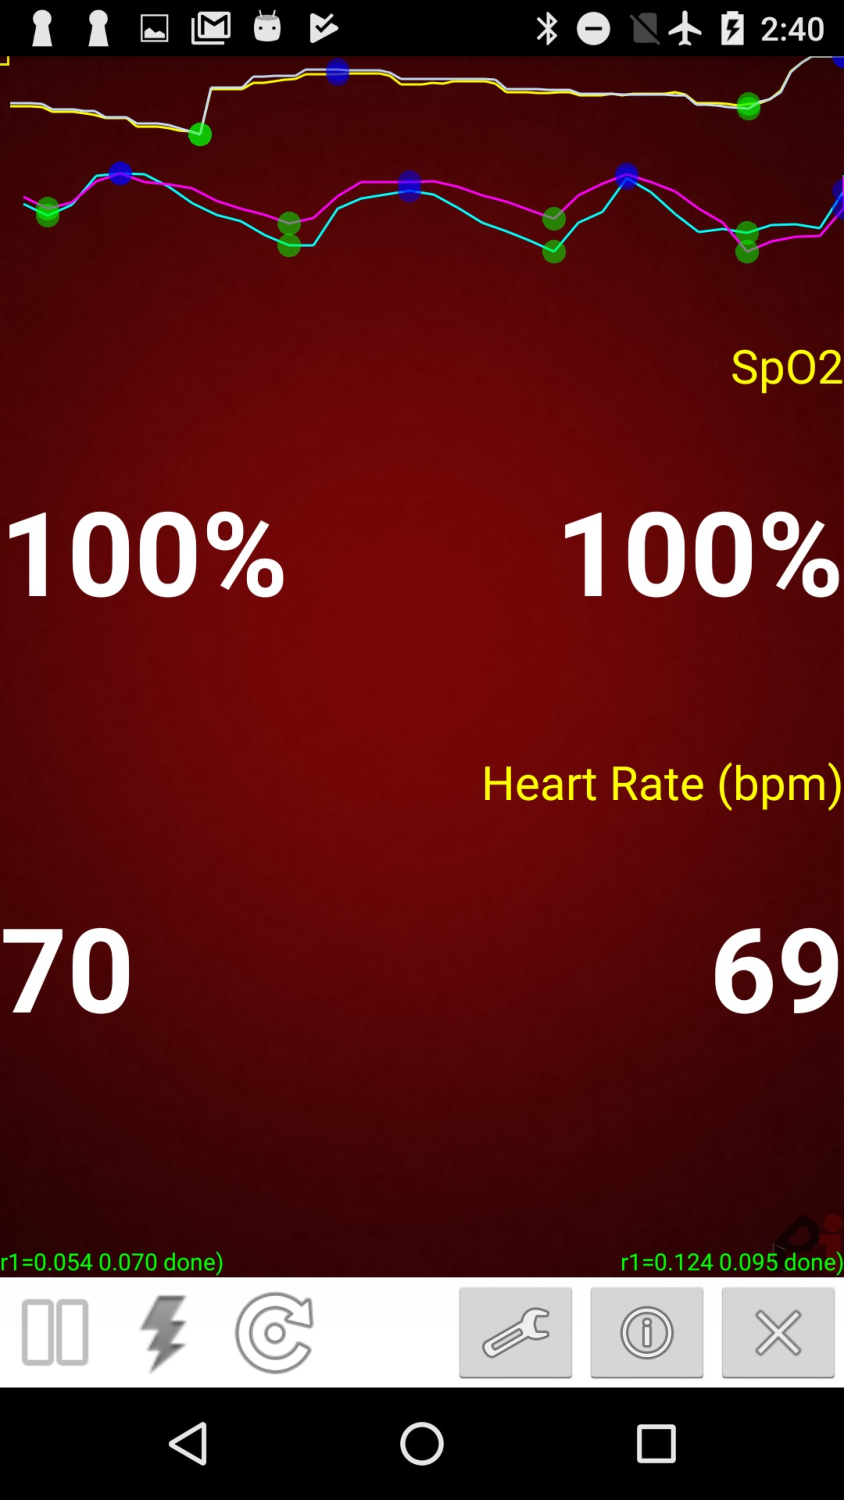
\includegraphics[height=6cm]{fig/moxi/moximeter.pdf}}
	\subfigure[]{\label{fig:D1D3}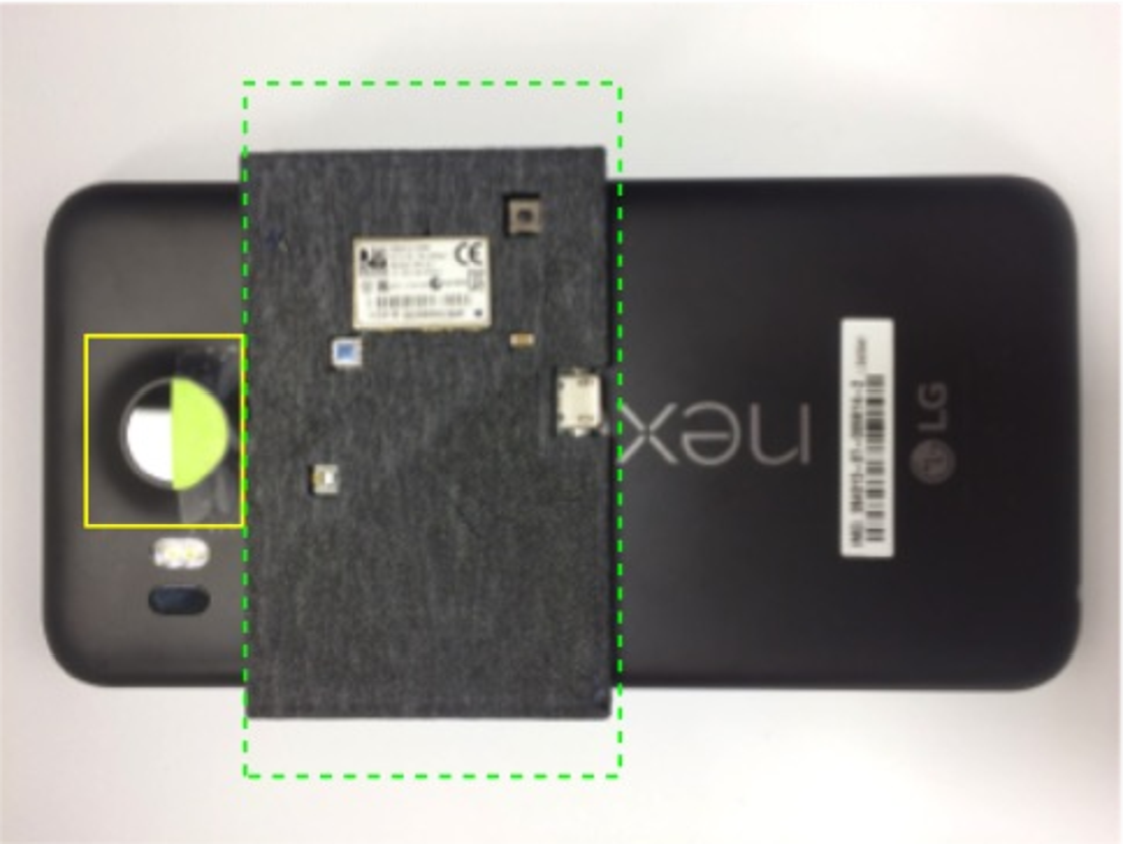
\includegraphics[height=6cm]{fig/moxi/D1D3.pdf}}
	\subfigure[]{\label{fig:D2}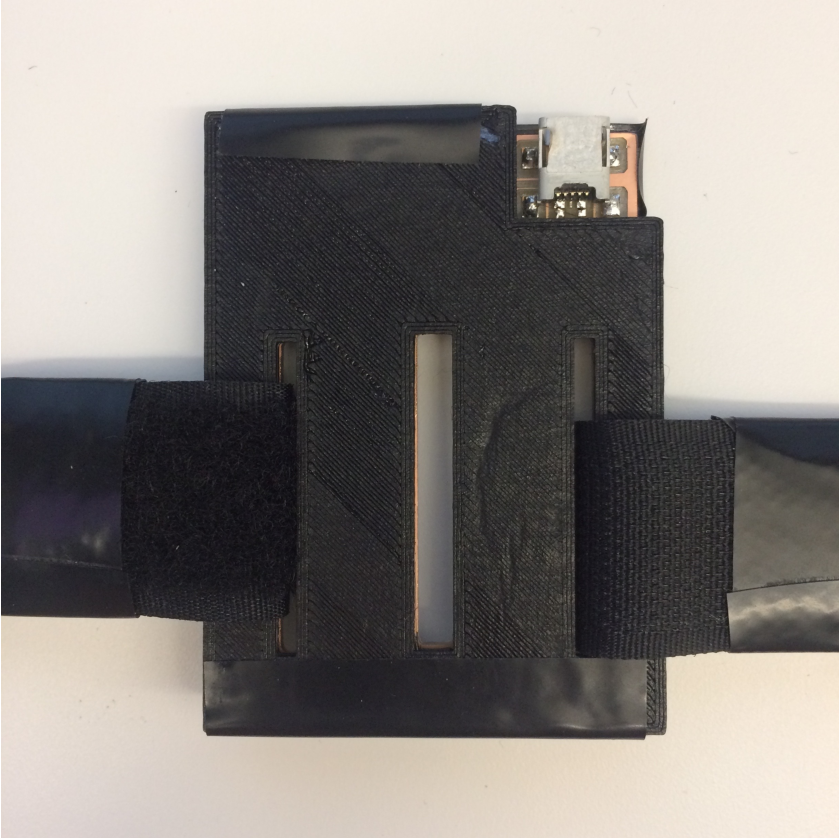
\includegraphics[height=6cm]{fig/moxi/D2.pdf}}
	\end{center}
	\caption{(a) Screenshot of Moximeter mobile application simultaneously capturing D1 and D3 data. (b) D1 (green, dashed) and D3 (yellow, solid) mounted on a smartphone phone. (c) D2 board with cover.} 
	\label{fig:designs}
\end{figure} 

In this chapter, we establish the feasibility and accuracy of three smartphone-based approaches to monitoring oxygenation. In order of decreasing complexity of hardware, the first design (D1) is a Bluetooth wireless oximeter board with a dedicated pulse oximetry chip [Figure~\ref{fig:D1D3}]. The second design (D2) measures tissue oxygen saturation (StO2). It functions by imaging light attenuation in tissue through a slit on a circuit board carrying LEDs [Figure~\ref{fig:D2}]. The third design (D3) is a paper filter covering half of the field of view of a smartphone camera [Figure~\ref{fig:D1D3}]. Both D1 and D3 designs utilize our in-house developed mobile phone application [Figure~\ref{fig:moximeter}] to monitor heart rate (HR) and arterial oxygen saturation (SpO2). The three devices, along with a screenshot of the mobile phone application, are seen in the figure below. Although we include details on D1 and D2 for completeness, when we refer to the \ac{MOXI} system, we are referring to the D3 design. 



%%% Section %%% 
\section{D1: Bluetooth Reflectance Pulse Oximeter}
\subsection{D1: Reflectance Board Hardware}
The D1 design works similarly to a clinical-quality pulse oximeter, except the optodes are placed on the same side of the finger. A photodiode captures the diffuse reflection of the light emitted from two on-board LEDs (640 and 940~nm) in order to estimate SpO2. This reduced form factor, non-finger-clip design makes pulse oximetry measurements more newborn friendly. The D1 board makes use of a low-cost (\$3.5 USD) dedicate pulse oximeter signal-processing chip (AFE4490 Integrated Analog Front-End, Texas Instruments, USA) and a microcontroller (ATMega32u4, Atmel, USA) communicating via the serial-peripheral interface (SPI) communication protocol. The 40x40~mm$^2$ rigid printed circuit board (PCB) can be battery powered or powered by a mobile phone using a male-to-male USB cable. 
    
\subsubsection{Optode settings for Neonates}
In reflectance measurements, the distance between the sources and detector determines the depth of photon propagation. Given the larger fingers of adults compared to neonates in our initial studies (MGH IRB approval is for use on adults with subsequent test on neonates), the current reflectance board has optodes optimized for an adult finger by using a large source-detector (SD) distance of 17~mm. This was empirically chosen based on sweeping the SD distance from 2.54 to 15.24~mm in 2.54~mm increments (0.1 inches to 0.6 inches in 0.1 inch increments based on the breakout board). The highest signal-to-noise ratio (SNR) at this distance was obtained when driving the LEDs at 25~mA. Both 10 mA and 50 mA resulted in smaller amplitudes of the AC component of the signals due to low photon detection and photodiode saturation, respectively. The same trend is seen with the SD distance where being too close or too far leads to weak signals or photodiode saturation. Although set to 17~mm for the pilot rests with adults, when used on neonates, the SD distance should be decreased to account for their smaller finger sizes. 

\subsubsection{Phone Mount}
\begin{figure}
    \begin{center}
    \subfigure[]{\label{fig:D1mount}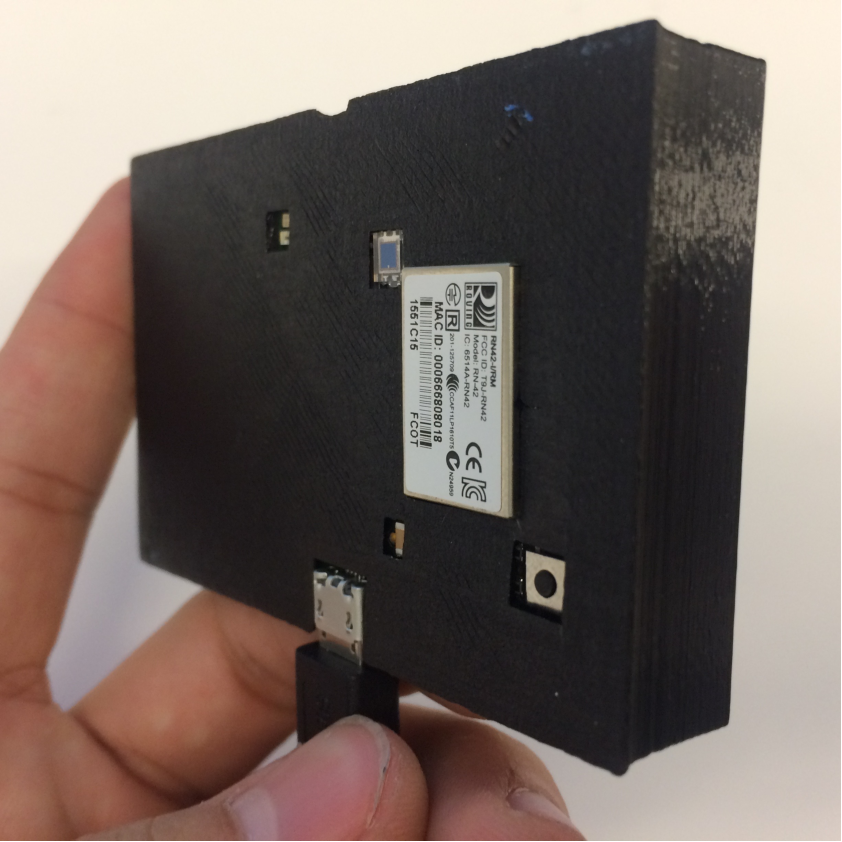
\includegraphics[height=5cm]{fig/moxi/D1mount.pdf}}
    \subfigure[]{\label{fig:D1D3mount}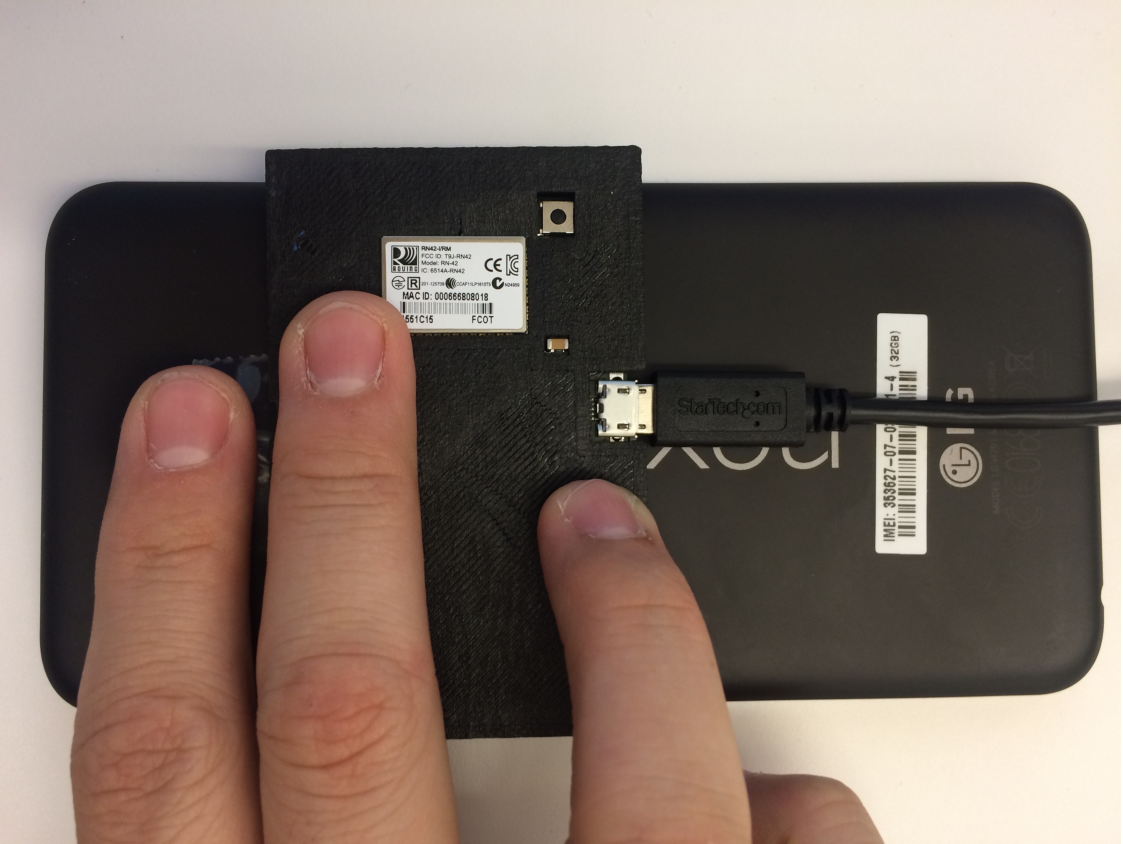
\includegraphics[height=5cm]{fig/moxi/D1D3mount.pdf}}
    \end{center}
    \caption{(a) D1 phone mount. (b) Simultaneous capture of D1 and D3.} 
    \label{fig:D1hardware}
\end{figure} 
The D1 board is placed over a Nexus 5X smartphone using a custom mount [Figure~\ref{fig:D1mount}]. The mount not only holds the D1 board onto the phone, but also prevents users from touching active electronics of the printed circuit board (PCB). The mount is 3-D printed out of Polylactic Acid (PLA). The side panels that grip onto the phone have gaps design to avoid accidentally pressing the volume and power buttons on the sides of the smartphone. The D1 board is press fit onto two small round tabs on the inside, eliminating the need for extra tools. The flat side of the mount is 0.2mm thick to allow maximum surface contact of the optodes onto the finger. Holes on the mount allow access to the reset button of the board, as well as allow the Bluetooth chip to protrude outside for better signal quality. The D1 board is mounted off center to the smartphone to accommodate the longer length of the middle finger compared to the index finger. This allows both fingers to lay comfortably flat during simultaneous capture of D1 and D3 signals [Figure~\ref{fig:D1D3mount}]. The D1 board is powered by a USB male-to-male cable connecting the board to the smartphone’s battery. 

\subsection{D1: Reflectance Board Software}
An Android phone application called Moximeter, written in Java, was developed to process the received signals from the D1 and display the results on the phone. Register values of the AFE4490 were set to 25 mA to each optode and a 500~Hz corner filter was applied post amplification. A long pulse repetition frequency of 250~Hz allows for dynamic averaging of 16 samples per data point by the analog-to-digital converter (ADC) to increase SNR. Bluetooth communication transmits data between the D1 board and the phone. The phone application displays the signals for the red and IR channels at the top of the screen. The signal sample-per-second (in Hz) is dynamically estimated and the PPG waveforms are process in real-time using embedded C-code for maximum efficiency to obtain the oxygen saturation values. The real-time signal processing includes a built-in signal filtering algorithm, peak detection, and algorithm to estimate HR, and an algorithm to compute SpO2 using a transmission pulse oximeter calibration model~\cite{Bailey2008}. The real-time HR and SpO2 values are displayed in the GUI [Figure~\ref{fig:moximeter}]. 
    
\subsubsection{Noise Removal}
Unlike a transmission finger clip where the optodes and finger are coupled, a reflectance-based measurement is more prone to noise and artifacts since the finger being sampled can move independently of the optodes. To reduce this noise, 16 readings of red and IR readings are sampled by the AFE4490 prior to sending an average value to Moximeter. The sampling is done on-board to maintain our 60~Hz sampling rate. Additionally, a 5~ms delay has been added between the SPI transfer calls by the microcontroller to allow the AFE4490 to stabilize. This stabilization prevents loss of data and decreases the likelihood of garbled measurements. As an added precaution, our processing of data workflow now incorporates a mean filter in addition to our band pass filter to remove any unwanted ``chirps'' or spikes in data. 
        
\subsubsection{Independent Source Control}
Photodiodes have a peak wavelength sensitivity and source-pairs have different power outputs from their red and IR LEDs for the same input current. Therefore, the ability to independently adjust each source transmission and receiving channel allows us to obtain comparable signals from the different optodes to increase the sensitivity of our SpO2 calculations.

The receiver channel of the AFE4490 is made up of a differential current-to-voltage trans-impedance amplifier followed by a current digital-to-analog converter (DAC). The amplifier has programmable a feedback resistor ($R_F$) and capacitor ($C_F$) to form a low-pass filter for the input signal current. The output voltage of the amplifier includes the AC component and a component resulting from ambient light leakage. The DAC attempts to amplify only the AC component of the pleth signal. By systematically varying $R_F$, $C_F$, DAC, and the transmitter reference voltage for each optode, we are able to determine the AFE4490 configuration that maximizes the AC components of both red and IR PPG signals, independently. Since the ratio-of-ratios, RR, is based on the amplitude of the AC component of the PPG signals, increasing the AC range with optimized AFE4490 configurations allows for more sensitivity in R calculations and thus more accuracy in SpO2 readings. 
        
\subsection{D1 Results}
\begin{figure}
    \begin{center}
    \subfigure[]{\label{fig:D1resultsa}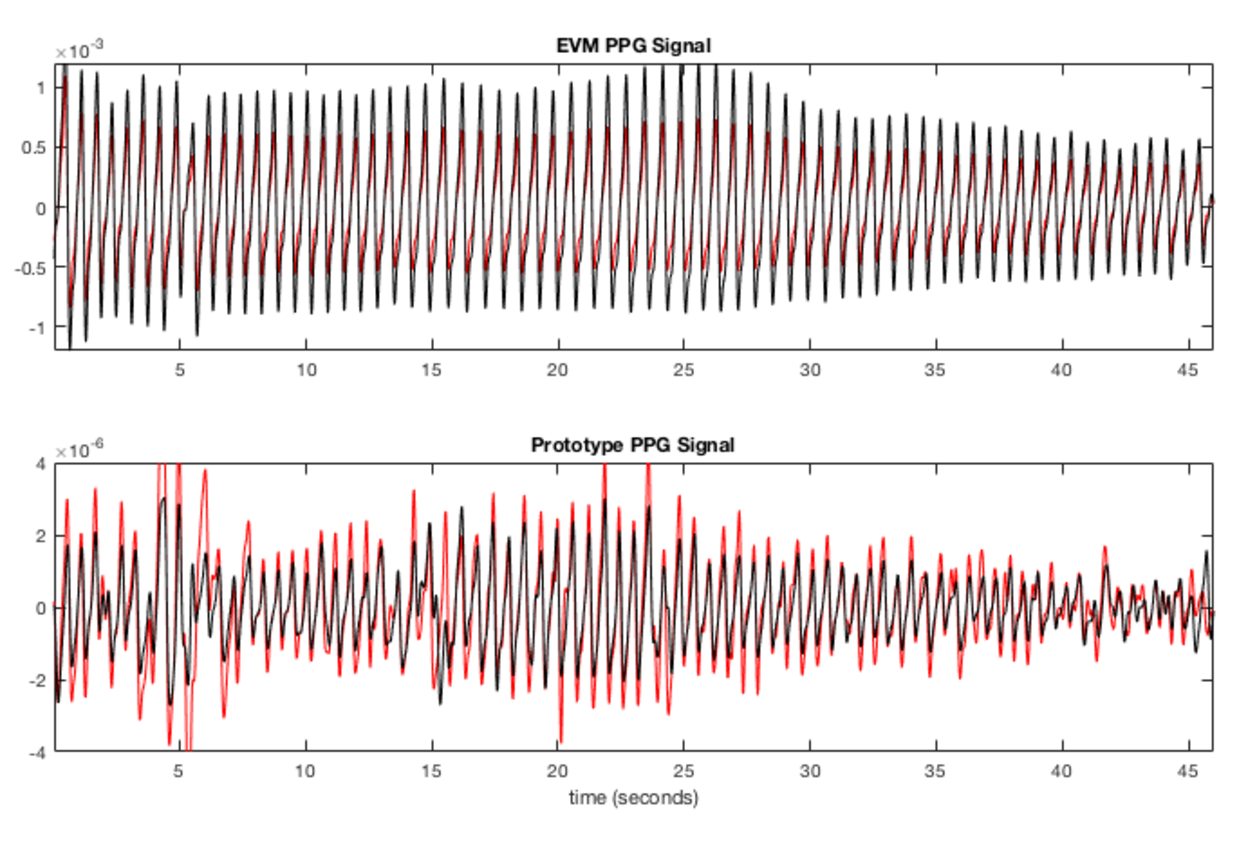
\includegraphics[width=.49\textwidth]{fig/moxi/D1resultsa.pdf}}
    \subfigure[]{\label{fig:D1resultsb}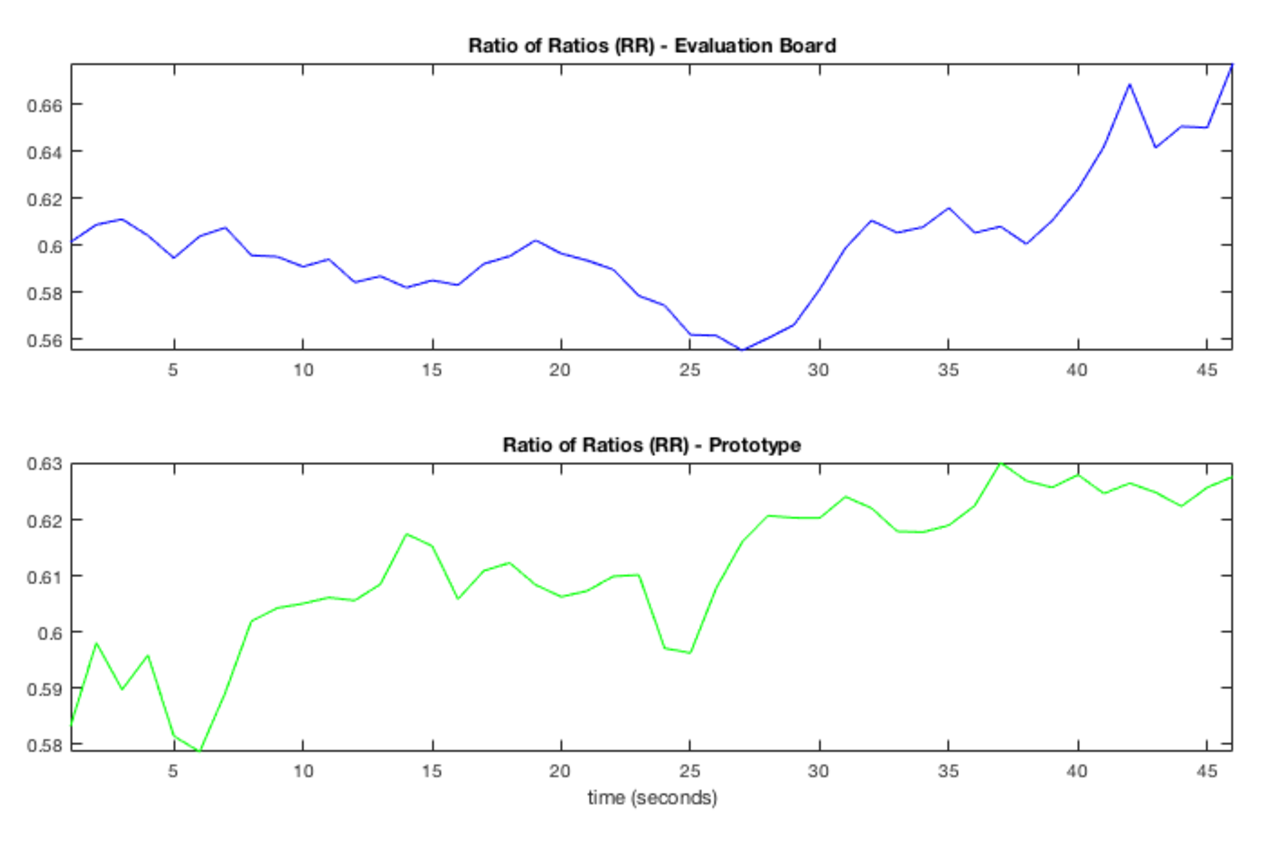
\includegraphics[width=.49\textwidth]{fig/moxi/D1resultsb.pdf}}
    \end{center}
    \caption{(a) EVM and prototype red (red) and infrared (black) PPG signals. (b) Ratio of Ratios in blue (EVM) and green (D1 Device).} 
    \label{fig:D1results}
\end{figure}
To evaluate the D1 prototype, we compared the obtained signals from our device against simultaneously acquired signals from the AFE EVM. The EVM captures PPG signals through transmission via a finger flip on the middle finger. The index finger of the same hand was placed over the optodes on the D1 device. The PPG signals in Figure~\ref{fig:D1resultsa} were simultaneously captured from the D1 device and from the AFE4490 EVM during a 46-second breath holding procedure. Signals were band-pass filtered using a sixth order zero-phase Butterworth filter to remove out of bound noise (0.2 to 5~Hz). As shown in Figure~\ref{fig:D1resultsb}, RR (Equation~\ref{eq:RR}) increases as SpO2 decreases due to the larger difference between extinction coefficients of HbO and HbR at red versus IR light. The pairwise linear correlation coefficient, R, between the two RR signals in Figure 7 is 0.4856. 



%%% Section %%%    
\section{D2: Single Slit Oximeter}
    \subsection{D2: Single Slit Hardware}
    \subsection{D2: Single Slit Software}
    \subsection{D2 Results}
        \subsubsection{Protocol}
        \subsubsection{Benchtop Results}



%%% Section %%% 
\section{D3: Paper Filter Pulse Oximeter (MOXI)}
    \subsection{Photon Propagation Simulations}
        \subsubsection{MCXlab simulations}
        \subsubsection{Optical Properties}
        \subsubsection{Attenuation Spectra of Paper Filters}
        \subsubsection{PPG Signal}
        \subsubsection{Ratio-of-ratio for broadband spectroscopy}
    \subsection{Simulation Validation Results}
    \subsection{Pilot clinical testing}
        \subsubsection{Breath-holding procedures}
        \subsubsection{Data Processing}
        \subsubsection{Pilot Test Results}



% --- EOF ---